\documentclass{article}
\usepackage[utf8]{inputenc}
\usepackage[T1]{fontenc} 
\usepackage[slovene]{babel} 

\usepackage{enumitem} 
\usepackage{hyperref}
\usepackage{amsmath}
\usepackage{amsthm} 
\usepackage{amssymb}
\usepackage{lmodern}
\usepackage{amsfonts} 
\usepackage{mathtools}
\usepackage{graphicx}
\usepackage{float}


\begin{document}

\title{Simetrična diskretna verižnica z liho členki\\
    \large Projekt pri predmetu Matematično modeliranje
}
\author{
    Matej Novoselec\\
}
\date{30.\ junij 2023}

\maketitle

\section{Uvod}
Projekt je sestavljen iz dveh delov - poročila in praktičnega dela, ki sestoji iz datotek v programskem jeziku Matlab.
V poročilu je le predstavljeno matematično ozadje problema in opis rešitve, do praktične rešitve problema in njegove vizualizacije pa se je možno dokopati z uporabo omenjenih datotek.
Pri vsakem delu poročila je po matematičnem razmisleku tudi navedeno, v kateri datoteki je rešitev zapisana/prikazana. 

\section{Problem diskretne verižnice}
Namen poglavja je povzeti postopek reševanja problema (splošne) diskretne verižnice, ki ga bomo nato ustrezno prilagodili zahtevam specifičnega problema v drugem poglavju poročila. 
Postopek reševanja je povzet po \cite{clanek}, kjer si ga bralec lahko tudi natančneje ogleda.
\newline
Imamo vrv, sestavljeno iz $n+1$ gibko vpetih togih členkov oziroma palic, katerih zaporedne dolžine so podane z
$$
L_{i},~i=1,~2,~ \ldots, ~n+1,
$$
mase členkov pa so podane z
$$
M_{i},~i=1,~2,~ \ldots, ~n+1.
$$
Podani imamo še robni točki verižnice oziroma obešališči, t.j. točki $(x_0,~y_0)$ in $(x_{n+1},~y_{n+1})$.
\newline
Določiti želimo koordinate (preostalih) krajišč, t.j. točk
$$
(x_{i},~y_{i}),~i=1,~2,~\ldots,~n,
$$
tako, da bo potencialna energija vrvi minimalna.
Pogoj za iskanje minimuma funkcije potencialne energije, t.j. funkcije
$$
F(x, y)=\sum_{i=1}^{n+1} M_{i} \frac{y_{i-1}+y_{i}}{2},
$$
se prek Pitagorovega izreka za vsako izmed palic prevede na iskanje vezanega ekstrema. 
Z uvedbo Lagrangeovih multiplikatorjev (označeni z $\lambda_{i}$) lahko iskanje vezanega ekstrema prevedemo na iskanje nevezanega, ter po standardnem postopku naredimo prehod na reševanje sistema (z $3n +1$ enačbami) oblike:
$$
\begin{aligned}
\lambda_{i}\left(x_{i}-x_{i-1}\right)-\lambda_{i+1}\left(x_{i+1}-x_{i}\right) & =0, \quad i=1,~2,~\ldots,~n, \\
\lambda_{i}\left(y_{i}-y_{i-1}\right)-\lambda_{i+1}\left(y_{i+1}-y_{i}\right) & =-\frac{M_{i}+M_{i+1}}{4}, \quad i=1,~2, ~\ldots, ~n, \\
\left(x_{i}-x_{i-1}\right)^{2}+\left(y_{i}-y_{i-1}\right)^{2} & =L_{i}^{2}, \quad i=1,~2,~\ldots,~n+1 .
\end{aligned}
$$
Reševanje sistema se lotimo z uvedbo relativnih koordinat:
$$
\begin{aligned}
& \xi_{i}=x_{i}-x_{i-1}, \quad i=1,~2,~\ldots,~n+1, \\
& \eta_{i}=y_{i}-y_{i-1}, \quad i=1,~2, \ldots,~n+1 \text {, }
\end{aligned}
$$
ki omogočajo zapis ekvivalentnega sistema:
$$
\begin{aligned}
\lambda_{i} \xi_{i}-\lambda_{i+1} \xi_{i+1} & =0, \quad i=1,~2, ~\ldots, ~n, \\
\lambda_{i} \eta_{i}-\lambda_{i+1} \eta_{i+1} & =-\frac{1}{2} \mu_{i}, \quad i=1,~2,~ \ldots,~ n, \\
\xi_{i}^{2}+\eta_{i}^{2} & =L_{i}^{2}, \quad i=1,~2, ~\ldots, ~n+1,
\end{aligned}
$$
kjer je
$$
\mu_{i}=\frac{M_{i}+M_{i+1}}{2}.
$$
Z nekaj računske manipulacije opazimo, da lahko zapišemo:
$$
\lambda_{i} \xi_{i}=-\frac{1}{2 u}, \quad i=1,~2,~\ldots,~n
$$
in
\begin{equation}
    \label{sim_lih}
    \frac{\eta_{i}}{\xi_{i}}=v-u \sum_{j=1}^{i-1} \mu_{j}, \quad i=1,~2,~\ldots,~n+1,
\end{equation}

kjer sta $u$ in $v= \frac{\eta_{1}}{\xi_{1}}$ neznani konstanti, iskanje katerih bo ključni korak postopka. 
\newline
Poskusimo izraziti $\xi_{i}$ in $\eta_{i}$ z $u$ in $v$, ter s tem pokažimo, da je dovolj poznati vrednosti teh konstant.
\newline
Z nekaj truda prek že dobljenih rezultatov zapišemo:
$$
1+\left(v-u \sum_{j=1}^{i-1} \mu_{j}\right)^{2}=\frac{L_{i}^{2}}{\xi_{i}^{2}},
$$
kar nam da predpis za $\xi_{i}$ v odvisnosti od neznanih konstant $u$ in $v$:
$$
\xi_{i} = \xi_{i}(u,~v)=\frac{L_{i}}{\sqrt{1+\left(v-u \sum_{j=1}^{i-1} \mu_{j}\right)^{2}}}, \quad i=1,~2,~\ldots,~n+1.
$$
Ker smo $\frac{\eta_{i}}{\xi_{i}}$ že izrazili z $u$ in $v$ je na dlani tudi zapis za $\eta_{i}$ v odvisnosti od neznanih konstant $u$ in $v$ (t.j. $\eta_{i} = \eta_{i}(u,~v)$).
\newline
Preostane nam torej le določiti konstanti $u$ in $v$, kar bomo storili prek sistema nelinearnih enačb:
\begin{equation}
    \label{sistem}
    \begin{aligned}
    U(u, v) & =\sum_{i=1}^{n+1} \xi_{i}(u,~v)-\left(x_{n+1}-x_{0}\right) = 0\\
    V(u, v) & =\sum_{i=1}^{n+1} \eta_{i}(u,~v)-\left(y_{n+1}-y_{0}\right) = 0.
    \end{aligned}
\end{equation}
Reševanje sistema se bomo lotili numerično, v programskem jezikom Matlab.

\section{Simetrična diskretna verižnica z liho členki}
Problem simetrične diskretne verižnice z lihim številom členkov,  je le redukcija problema (splošne) diskretne verižnice.
\newline
K zahtevam prvotnega problema dodamo pogoj za simetričnost, ki narekuje 
$$ 
y_0 = y_{n+1}~~\text{in}~~L_1 = L_{n+1},~L_2 = L_n,~\dots;~L_i = L_{n+2 - i},
$$
ter pogoj za lihost, ki je izpoljen, če velja $n + 1 = 2 l +1~\text{oziroma}~l = \frac{n}{2}$.
\newline
Prednost pri reševanju tako zastavljenega problema, v primerjavi z reševanjem problema splošne diskretne verižnice, je ta, da dodatno zahtevani pogoji implicirajo vodoravno lego sredinskega členka diskretne verižnice, t.j. velja $y_{l} = y_{l+1}$.
Ob ogledu enačbe (\ref{sim_lih}) opazimo, da to implicira:
$$
    \eta_{l+1} = \xi_{l+1} \bigg(v - u \sum_{j = 1}^{l} \mu_{j} \bigg) = 0, 
$$
kar omogoča izražavo iskane spremenljivke $v$ z iskano spremenljivko $u$ kot:
$$
v = u \sum_{j = 1}^{l} \mu_{j}.
$$
To lahko sedaj vstavimo v sistem nelinearnih enačb iz postopka reševanja problema splošne diskretne verižnice, ter dobimo sistem dveh nelinearnih enačb z eno neznanko (iskanim $u$-jem). 
Da $u$ (in posledično $v$) določimo, je torej dovolj rešiti eno nelinearno enačbo (v našem primeru bo to enačba za $U$).
\newline
Predpis za nelinenarno enačbo se iz (\ref{sistem}) glasi:
$$
0 = U(u,~u \sum_{j = 1}^{l} \mu_{j}) = \sum_{i=1}^{n+1} \xi_{i}\big(u,~u \sum_{j = 1}^{l} \mu_{j}\big)-(x_{n+1}-x_{0}) =: f(u).
$$
Reševanje nelinearne enačbe se lotimo numerično s pomočjo metode $fsolve$ v programskem jeziku matlab.
Tako dobimo (približek za) rešitev $u$ (in posledično $v$), ki nam bo omogočala izražavo koordinat/vozlišč členkov naše diskretne verižnice.
Postopek je povsem enak tistemu iz splošne diskretne verižnice, bralec si ga lahko natančneje ogleda v \cite{clanek}.
\newline
Postopek redukcije na reševanje ene nelinearne enačbe (za $u$) ja na zgoraj zapisan način izveden/zapisan tudi v priloženih datotekah $enacba\_za\_U.m$ (ki nastavi nelinearno enačbo), ter $sim\_disk\_ver\_liho\_clenkov.m$ (ki enačbo reši in poračuna vozlišča členkov verižnice).
\newline
Spodnja slika prikazuje rešitev problema simetrične diskretne verižnice z liho členki z začetnimi podatki problema $(x_0,~ y_0) = (0,~0),~(x_{n+1},~y_{n+1}) = (5,~0)$ in $L = [2~1~2~1~2~1~2]$, ter $M = [2~1~2~1~2~1~2]$. 

\begin{figure}[H]
    \begin{center}
    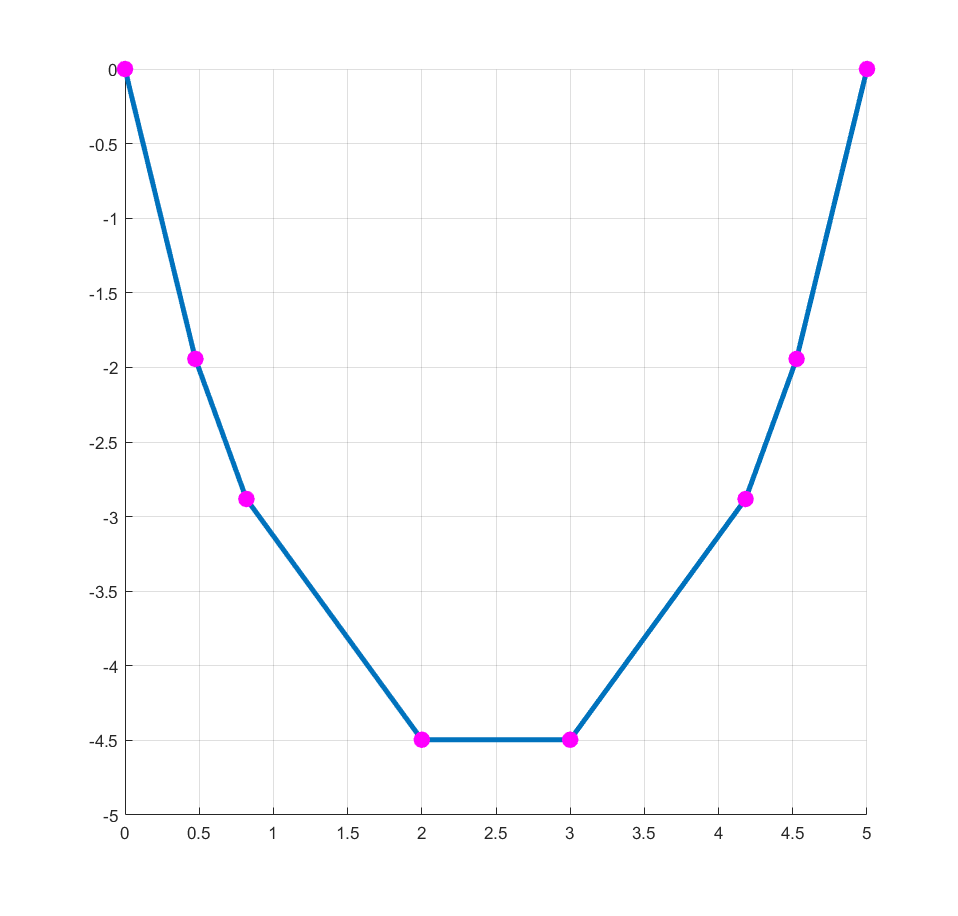
\includegraphics[width=350pt]{disk_ver.png}
    \caption{Simetrična diskretna verižnica z liho členki}
    \end{center}    
\end{figure}

Bralec si lahko kodo za izris ogleda v datoteki $risi\_liha\_simetricna\_veriznica.m$ in spremeni vhodne podatke problema v datoteki $test\_liha\_simetricna\_disk\_ver.m$.

\pagebreak 

\section{Odboji lahke žogice po diskretni verižnici}
Ko določimo vsa vozlišča diskretne verižnice, v izbrani začetni točki (označimo s $s_0 = (s_x,~s_y)$) z začetno hitrostjo (označimo z $v_0 = (v_x,~v_y)$) spustimo lahko kroglico, da se le-ta odbija od naše diskretne verižnice. 
Zanima nas, kje se žogica nahaja po $n$ odbojih.
\newline
Vredno je omeniti, da nam predpostavka, da je žogica lahka implicira, da na njo ne deluje zračni upor in da se pri trku z verižnico energija ohranja oziroma je trk elastičen (t.j. vhodni in izhodni kot odboja sta enako velika).
\newline
Problema se lotimo v dveh korakih. V prvem koraku želimo iz dobljenih vozlišč diskretne verižnice, konstruirati funkcijo, katere graf bo na intervalu $[x_0,~x_{n+1}]$ sovpadal z diskretno verižnico, t.j. poiščemo odsekoma linearno funkcijo (linearna na intervalih $[x_i,~x_{i+1}]$), ki se bo na vsakem linearnem odseku ujemala z ustreznim členkom diskretne verižnice. 
Ko določimo še trajektorijo žogice, bomo s tako konstruirano funkcijo lahko numerično iskali točko odboja kot točko preseka omenjenih predpisov. 
\newline
Z $(x_i, ~y_i)$ označimo $i$-to zaporedno vozlišče diskretne verižnice in definirajmo "funkcijo":
$$
    F(x) = \begin{cases}
        \frac{y_{i+1} - y_i}{x_{i+1} - x_i}(x - x_i) + y_i~;~~ x \in [x_i,~ x_{i+1}]~\text{za}~ i=0,~1,~\dots,~n\\
        "\infty"~;~~\text{sicer}
    \end{cases}.
$$
Zapisali smo funkcijo, katere graf predstavlja diskretno verižnico. Oglejmo si še trajektorijo lahke žogice (brez odbojev). 
Na gibanje vpliva le gravitacijski pospešek ($g = 9.81$), zato je trajektorija podana z:
$$
\begin{bmatrix}
    x(t) \\
    y(t)
\end{bmatrix} =
\begin{bmatrix}
    s_x \\
    s_y
\end{bmatrix} + 
\begin{bmatrix}
    v_x \\
    v_y
\end{bmatrix} t - \frac{1}{2}
\begin{bmatrix}
    0\\
    g
\end{bmatrix} t^2,
$$
njena hitrost pa z:
$$
\begin{bmatrix}
    \dot{x}(t) \\
    \dot{y}(t)
\end{bmatrix} =
\begin{bmatrix}
    v_x \\
    v_y
\end{bmatrix} - 
\begin{bmatrix}
    0\\
    g
\end{bmatrix} t.
$$
Sedaj lahko iščemo čas potovanja žogice po trajektoriji (od začetka) do presečišča z funkcijo, ki podaja diskretno verižnico. Ravno presečišče bo točka na diskretni verižnici, od katere se bo žogica odbila. 
Problema se lotimo numerično, z metodo $fsolve$. Poiščemo točko presečišča oziroma odboja, čas do tega presečišča, ter hitrost žogice, s katero prileti na odbojno mesto na verižnici. 
Če ugotovimo, da presečišče ne obstaja, to pomeni da se žogica od verižnice (več) ne odbije.
\newline
Za konec prvega koraka omenimo, da si bralec nastavek funkcije $F$ lahko ogleda v datoteki $funkcija\_veriznica.m$, koda za iskanje presečišča in podatkov o presečišču pa je spisana v datoteki $presek\_funkcija\_v\_pot\_zogice.m$.
\newline
\newline
Opremljeni s podatki o presečišču oziroma odbojnem mestu, se lotimo drugega koraka. 
Želeli bi poračunati vektor hitrosti žogice po odboju od členka diskretne verižnice. Iz prvega koraka poznamo točko odboja in hitrost tik pred odbojem (označimo z $\vec{v}$). Prek točke odboja lahko določimo členek, od katerega se bomo odbili, ter tako tudi normalo na ta členek (označimo z $\vec{n}$).
Vektor hitrosti po odboju (označimo z $\vec{w}$) lahko tako določimo prek formule $\vec{w} = \vec{v} - 2 \frac{\vec{v} \cdot \vec{n}}{||\vec{n}||^2} \vec{n}$.
\newline
Opazimo, da smo sedaj problem položaja po $n$-tih odbojih prevedli na problem položaja po $(n-1)$-tih odbojih, če za nov začeten položaj vzamemo točko (zadnjega) odboja, za novo začetno hitrost pa hitrost žogice po odboju. 
\newline
Opisan postopek drugega koraka, oziroma izvedbo enega odboja, si lahko bralec ogleda v datoteki $odboj\_funkcija\_disk\_ver.m$, priloženi pa sta tudi pomožni funkciji za vektor hitrosti po odboju ($odboj.m$) in funkcija, ki poišče normalo na členek ($normala\_na\_clenek.m$).
\newline
\newline
Kot že zapisano, lahko sedaj določimo položaj po $n$-tih odboji, tako da $n$-krat ponovimo postopek za iskanje odboja. To delo numerično namesto nas opravi priložena datoteka $n\_odbojev\_zogica.m$.
\newline
\newline
Na spodnji sliki je izrisanih prvih sedem odbojev lahke žogice, ki jo z začetno hitrostjo $\vec{v} = (2,~1)$ pošljemo iz začetne točke $(3, ~-1/2)$.
Rdeče točke nakazujejo točke odbojev, pot žogice med njimi pa je obarvana z zeleno. Modra točka nakazuje gibanje žogice po zadnjem odboju.

\begin{figure}[H]
    \begin{center}
    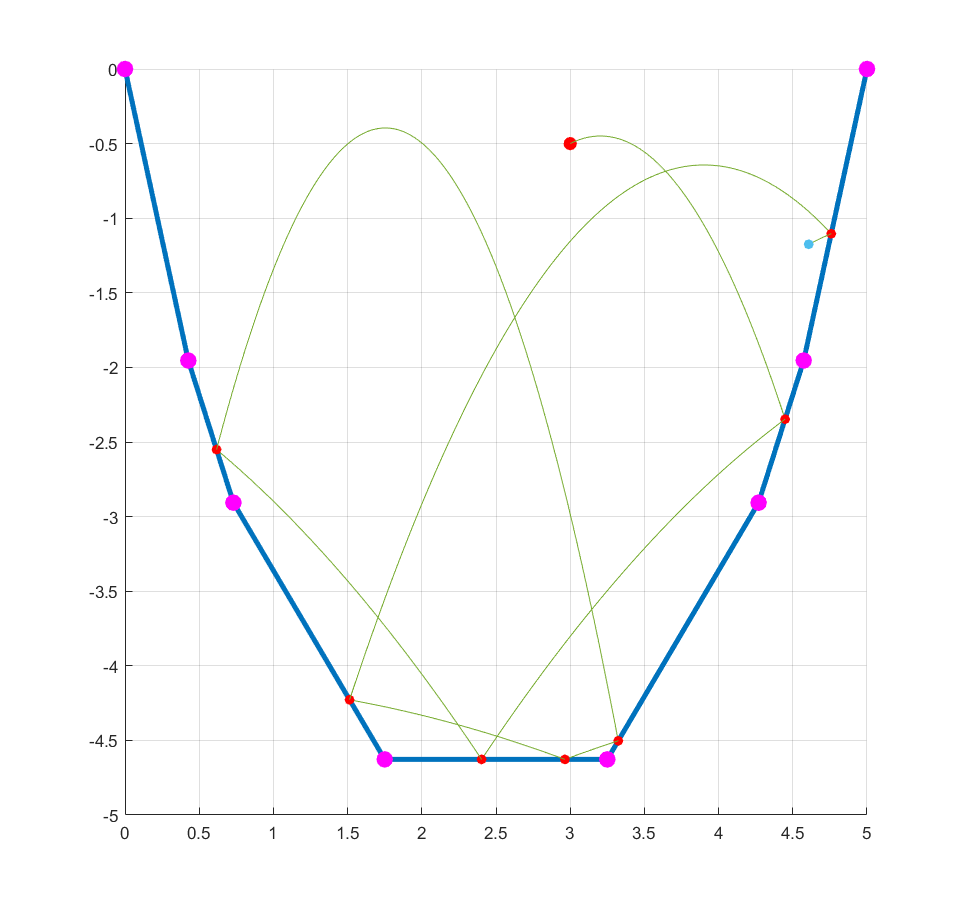
\includegraphics[width=280pt]{odboji.png}
    \caption{Odboji na simetrični diskretni verižnici z liho mnogo členki}
    \end{center}    
\end{figure}

Naslednje slika prikazuje primer večjega števila odbojev in členkov.

\begin{figure}[H]
    \begin{center}
    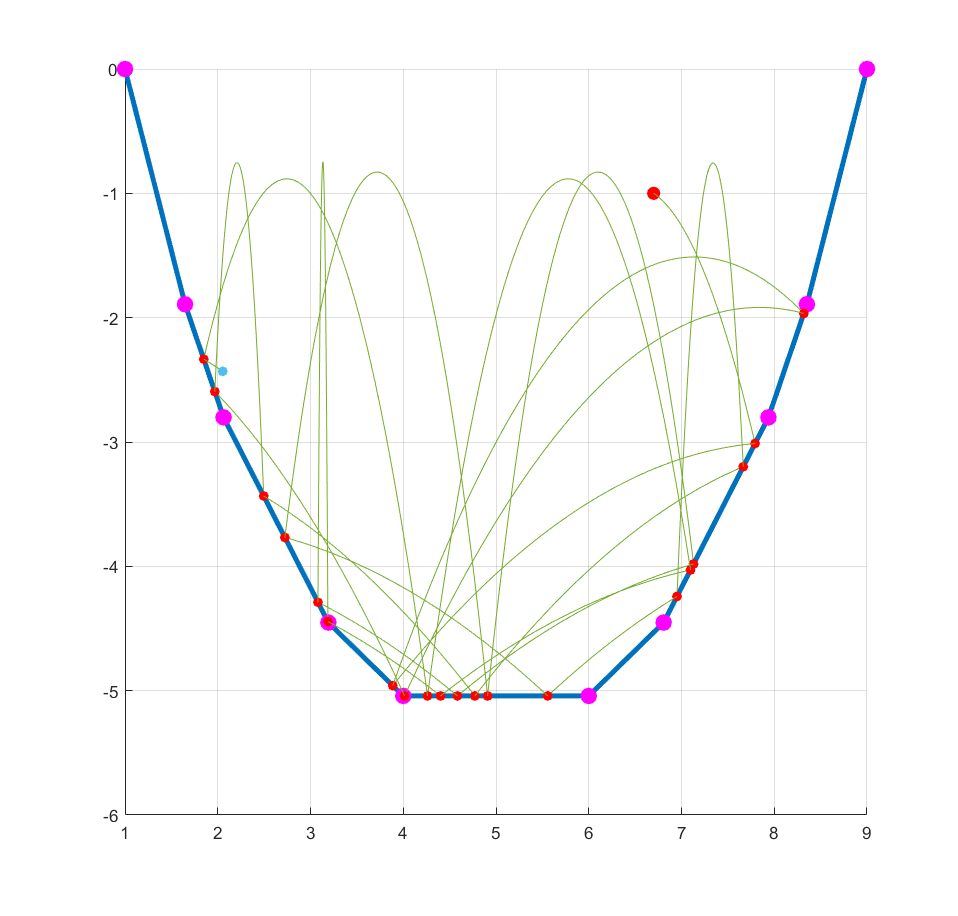
\includegraphics[width=320pt]{odboji_vec.png}
    \caption{Večje število odbojev na diskretni verižnici}
    \end{center}    
\end{figure}

Bralec si kodo za animacijo in izris lahko ogleda v datoteki $risi\_odboji\_gravitacija.m$, ter spremeni vhodne podatke v datoteki $test\_odboji\_gravitacija.m$.

\bibliographystyle{siam}
\begin{thebibliography}{9}
    \bibitem{clanek}
        E.~Zakrajšek, \emph{Verižnica}, [ogled 30.~6.~2023], dostopno na \url{https://ucilnica.fmf.uni-lj.si/pluginfile.php/8283/mod_resource/conte4/predavanja/veriznica/veriznica.pdf}.
    \bibitem{zapiski}
        E. Žagar \emph{Zapiski predavanj 22.3.2021 - Problem diskretne verižnice} [ogled 29.~6.~2023], dostopno na \url{https://ucilnica.fmf.uni-lj.si/pluginfile.php/100122/mod_resource/content/1/mm_uni_22_3_21.pdf}.
\end{thebibliography}

\end{document}